% ==========================================================================
% Two geographies of urban deprivation — PNAS-format version (8-page target)
%
% Condensed from ../main.tex (the full-length draft, which stays the master
% for Overleaf revisions). Same numbers, same sources (docs/paper-pack/data,
% audited by tools/audit_paper_pack.py); moved material lives in si.tex.
% Figures are re-rendered at PNAS column widths by make_figs_print.py.
% Layout mimics PNAS two-column metrics (17.8 cm text width, 8.7 cm
% columns, 9 pt) for page estimation; swap for pnas-new.cls at submission.
% ==========================================================================
\documentclass[9pt,twocolumn]{article}

\usepackage[T1]{fontenc}
\usepackage[utf8]{inputenc}
\usepackage{lmodern}
\usepackage[paperwidth=21cm,paperheight=27.9cm,textwidth=17.8cm,textheight=23.5cm,columnsep=0.45cm]{geometry}
\usepackage{graphicx}
\usepackage{booktabs}
\usepackage{amsmath}
\usepackage{caption}
\usepackage[numbers,sort&compress]{natbib}
\usepackage[hidelinks]{hyperref}
\usepackage{url}
\usepackage{float}

\newcommand{\doi}[1]{doi:~\href{https://doi.org/#1}{\nolinkurl{#1}}}
\graphicspath{{figures/}}
\captionsetup{font=footnotesize,labelfont=bf,skip=4pt}
\setlength{\parskip}{0pt}
\newcommand{\gref}{g(15)}
\newcommand{\pw}[1]{$p_{\mathrm{wild}} = #1$}
\newcommand{\pperm}[1]{$p_{\mathrm{perm}} = #1$}

\title{\textbf{Two geographies of urban deprivation: everyday services and
emergency care across European cities}}
\author{Tina Comes$^{1,\ast}$\\[2pt]
  \small $^{1}$Delft University of Technology, Faculty of Technology, Policy and Management, Delft, The Netherlands\\
  \small $^{\ast}$Corresponding author: \texttt{t.comes@tudelft.nl} \quad
  \emph{[Author list and affiliations to be completed.]}}
\date{}

\begin{document}

\twocolumn[
\maketitle
\begin{minipage}{\textwidth}
\small
\noindent\textbf{Abstract.}
Proximity has become the planning paradigm of European cities: the
15-minute city promises every daily need within a short walk and is
advanced as a route to urban resilience. That promise concerns everyday
life. Urban populations also face a growing burden of emergencies, with
heat alone killing an estimated 44,000 Europeans a year and the number
exposed to extreme heat projected to rise from ten million to almost 300
million a year under three degrees of warming; in an emergency what
matters is whether care reaches people in time. Accessibility research
measures both kinds of need as travel time, which cannot say how much a
resident loses when a service lies further away. Deprivation theory,
developed in humanitarian logistics to quantify the welfare lost during
time without an essential good, can. We bring that theory into urban
analysis and ask whether the deprivation cities impose follows the same law
for everyday and for emergency needs. Measuring both on a 100\,m population
grid for 67 functional urban areas in 24 European countries, we find two
regimes that obey different laws. Everyday deprivation falls with city
size while emergency deprivation does not, and everyday inequality widens
with size while emergency inequality never narrows. Emergency deprivation
follows the coverage of national emergency systems rather than city size:
five cities that appear average by travel time carry 2.4 to 4.7 times the
typical emergency deprivation. Within cities, the neighbourhoods most
deprived of everyday services are also, more often than chance, the most
deprived of emergency care, and neighbourhoods with many children carry
this compounded deprivation most consistently. A city that works every day
is not thereby resilient.

\medskip
\noindent\textbf{Significance.}
Cities are planned for everyday proximity, yet urban populations
increasingly face emergencies in which minutes decide survival. We show
that everyday and emergency needs form two regimes of urban deprivation
that obey different laws. Measuring anchored deprivation rather than
travel time across 67 European city regions, larger cities reduce everyday
deprivation but not emergency deprivation, everyday inequality grows with
city size, and emergency deprivation follows national coverage, with five
capitals harbouring emergency deserts that travel-time averages cannot
detect. The same neighbourhoods, often those with many children, lose in
both regimes. A city that works every day is not thereby resilient;
urban resilience requires both regimes.

\medskip
\noindent\textbf{Keywords:} urban deprivation; accessibility; 15-minute
city; emergency medical services; urban resilience; spatial equity; urban
scaling
\vspace{10pt}
\end{minipage}
]

% ==========================================================================
\section*{Introduction}
% ==========================================================================

Three quarters of Europeans live in urban areas, a share projected to
exceed 83\,\% by 2050 \citep{eea2024urbanadaptation}, and the cities they
live in are increasingly planned around one idea: that every daily need
should lie within a short walk. The 15-minute city has become the planning
paradigm of the continent \citep{moreno2021fifteenminute,allam2022fifteenminute},
and it describes an everyday regime, in which residents choose when to
reach a general practitioner, a pharmacy, a supermarket, a school or a
park. Urban life is also lived in a second regime. Heat kills an estimated
44,000 Europeans a year, a toll projected to triple by 2100 under current
policies \citep{garcialeon2024mortality}, and the number exposed to
extreme heat rises from about ten million a year today to almost 300
million under three degrees of warming \citep{naumann2020heat}. The
emergency regime is exercised every day and not only in disasters: across
Europe about 8\,\% of people who suffer a cardiac arrest outside hospital
survive, the ambulance reaches them after 12 minutes on average, and each
minute of delay lowers the probability of survival
\citep{grasner2020eureca,grasner2025eureca3,larsen1993survival}. The
European Union now asks member states to plan for emergencies explicitly
\citep{ec2025preparedness}. Everyday life and emergencies place different
demands on the same city. What does a resident lose when the services they
need lie further away, and does the answer differ between the everyday
and the emergency regime?

Urban research has one established answer, and it is a measurement rather
than a theory. Accessibility, defined by Hansen as ``a measurement of the
spatial distribution of activities about a point''
\citep{hansen1959accessibility}, is operationalised as travel time. The
15-minute-city programme \citep{moreno2021fifteenminute,papadopoulos2023compliance},
global travel-time mapping \citep{weiss2020healthcare,wu2025global} and
the measurement of unequal access within cities
\citep{nicoletti2023disadvantaged} all count minutes, and a minute counts
the same wherever it falls, for whichever service, for whichever
resident. Combined with urban scaling, whose empirical regularity
\citep{bettencourt2007growth} and generative theory
\citep{bettencourt2013origins} hold that infrastructure and services
improve systematically with city size, the access position implies a
prediction: larger cities should serve every need better, everyday and
emergency alike. The position has no reason to expect two service
classes to behave differently.

Welfare economics offers a second position. Deprivation theory, developed
in humanitarian logistics, defines the deprivation cost of a good as the
welfare lost during the time a person spends without it, and shows that
this cost is estimable as a function of deprivation time
\citep{holguinveras2013objective,holguinveras2016econometric}. Two objects
follow, and their difference carries this paper. For substitutable goods
the loss is a \emph{level}: bounded and S-shaped, saturating once people
adapt and substitute \citep{wang2017deprivation}. For critical goods the
loss is a \emph{cost}: convex and unbounded, rising ever more steeply with
time, with estimates for goods and for emergency ambulance services
\citep{cantillo2018discrete,macea2018attitudes,delgadolindeman2019ambulance}.
The value of time of transport economics, estimated on routine trips
whose delay can be rescheduled, is the wrong valuation for the second
object: the clinical evidence that survival after cardiac arrest falls by
one to two percentage points per minute of delay
\citep{larsen1993survival,nicholl2007distance} is a statement about
mortality. Deprivation theory therefore predicts what the access position
cannot: because the welfare lost follows the need, the two regimes need
not obey the same law, and a city may serve one while failing the other.
Urban resilience research reaches the same distinction from the other
side: resilience is defined through equitable access to essential
services \citep{meerow2016defining,logan2020reframing}, the 15-minute city
is advanced as a resilience strategy \citep{moreno2021fifteenminute}, yet
everyday vulnerability profiles fail as predictors of crisis-time
capability \citep{sirenko2026heatwaves}, and whether the neighbourhoods a
city fails every day are also those it fails in an emergency
\citep{cutter2003vulnerability} is an open empirical question.

The stakes are not academic. By the standard access statistic, the median
drive time to emergency care, Bucharest is served better than the typical
European city (8.5 minutes, 0.71 times the sample median). By deprivation
cost it carries 2.8 times the typical burden, because a well-served core
pulls the median down while a deep periphery lies far beyond any clinical
response benchmark. Which number a planner sees decides whether Bucharest
has an emergency problem at all. In this paper we measure which of the two
positions describes urban Europe.

We do so for 67 functional urban areas (FUAs) in 24 European countries,
from 101{,}050 to 12.9 million inhabitants, drawn by a stratified design
over four macro-regions and four size strata, on a common 100\,m
population grid. Europe is the setting for three reasons. It has a
harmonised functional city definition \citep{dijkstra2019fua}, a
harmonised census grid, near-complete street and facility mapping, and
clinical emergency-response benchmarks shared across national systems
\citep{pons2005response,blanchard2012response,peleg2004ems}, which global
travel-time mapping \citep{weiss2020healthcare,wu2025global} cannot carry.
It is the mature end of the urban life cycle in which large cities lose
their growth advantage \citep{musso2026cities}, so its cross-sectional
size gradient reads what size delivers once growth no longer favours the
large city. And access to essential services is a right in the European
legal order \citep{eu2012charter,eu2017pillar}, with emergency care
organised nationally under shared response targets, so the sample covers
one polity with one set of obligations and 24 national emergency systems.
Following the scaling tradition we estimate log-log elasticities of city
outcomes on population \citep{bettencourt2007growth}; every size gradient
is cross-sectional, and ``as cities grow'' means the space-for-time reading
of that gradient, never a longitudinal observation.

Three findings follow. First, deprivation is a different object from
access: it explains the cross-city structure better than travel time,
agrees with travel time wherever results are rank-based, and reveals what
travel-time averages hide, five emergency deserts in European capitals.
Second, urban growth delivers on one clock only: everyday deprivation falls
with city size and emergency deprivation does not, everyday inequality
widens with size and emergency inequality never narrows, and emergency
deprivation follows the coverage of national emergency systems rather than
city size. Third, the two deprivations compound: in 66 of 67 cities the
neighbourhoods most deprived of everyday services are also, more often
than chance, the most deprived of emergency care, and neighbourhoods with
many children carry the compounded burden most consistently.

% ==========================================================================
\section*{Results}
% ==========================================================================

Two surfaces summarise each city (Fig.~\ref{fig:curves}; Materials and
Methods). The \emph{everyday deprivation level} of a grid cell, between 0
and 1, expresses how far the burden of reaching five everyday service
categories on foot has progressed toward saturation: near 0, all services
are comfortably walkable; near 1, additional minutes no longer add burden.
The \emph{emergency deprivation cost} of a cell is an open-ended positive
number expressing the welfare lost through its drive time to the nearest
emergency facility, in multiples of the loss at the 15-minute
emergency-medical-service (EMS) benchmark: a cell at 2.0 carries twice the
deprivation of one whose ambulance arrives at the benchmark, and the cost
keeps escalating beyond it. ``Cost'' is welfare lost, never money, and
deprivation throughout is the welfare loss imposed by poor physical
access, distinct from the socioeconomic deprivation of composite indices,
which enters only as an explanatory variable. The two objects differ
because the needs do: everyday services can be substituted or deferred,
so the marginal minute loses value once coping sets in and the loss is
bounded; emergency care cannot, survival worsens with every minute, so
the marginal minute gains value and the loss is unbounded. The linear loss of a travel-time average over-prices minutes where they
are welfare-inert and under-prices them where they are clinically
decisive. One discipline follows: only unit-invariant statistics (elasticities,
Ginis, ranks) cross regimes, and raw magnitudes never do.
Table~\ref{tab:sample} summarises the sample. Cities nest in 24
countries, so every scaling claim cites a wild cluster bootstrap p-value
on country clusters and every regional contrast a country-permutation
p-value.

\begin{figure*}[t]
\centering
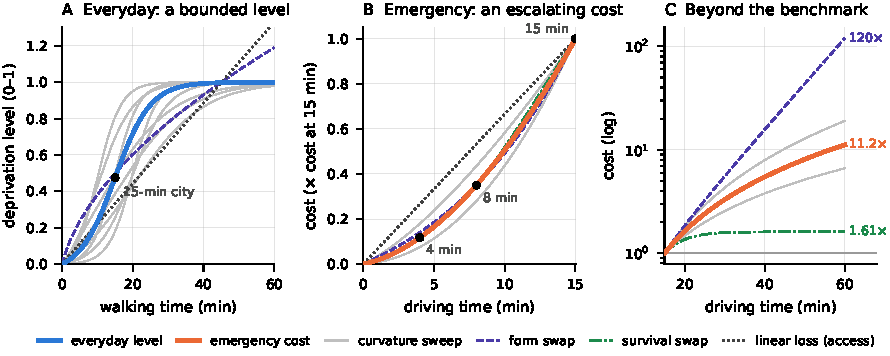
\includegraphics[width=\textwidth]{fig1_curves.pdf}
\caption{The two deprivation functions. (A) Everyday deprivation level
against walking time: bounded, saturating, inflection at the 15-minute
anchor. (B) Emergency deprivation cost against driving time inside the
benchmark window, in multiples of the cost at the 15-minute EMS target;
all forms coincide at the clinical anchors (4, 8, 15 min) by
construction. (C) Beyond the target no benchmark exists and three
escalation hypotheses diverge (log scale). Grey: curvature sweep; dashed:
form swaps (SI Appendix); dotted: the linear loss a travel-time average
implies. Panels are on different scales.}
\label{fig:curves}
\end{figure*}

\begin{table}[t]
\centering
\caption{Sample by macro-region: 67 functional urban areas (Eurostat/OECD
definition), stratified over 4 regions $\times$ 4 size strata, 113.9
million residents. $\bar D_{\mathrm{ev}}$: mean everyday deprivation
level; $\bar C_{\mathrm{em}}$: mean emergency deprivation cost (multiples
of \gref{}; not comparable in magnitude); $\rho$: rank coupling of the
two surfaces; HH: compounding share at the median split. Full per-city
table in SI Appendix.}
\label{tab:sample}
\footnotesize
\setlength{\tabcolsep}{3.5pt}
\begin{tabular}{@{}lrrrrrrr@{}}
\toprule
Region & Cities & Countries & Pop.\ (M) & $\bar D_{\mathrm{ev}}$ & $\bar C_{\mathrm{em}}$ & $\rho$ & HH \\
\midrule
North  & 13 & 4  & 11.3 & 0.41 & 1.81 & 0.47 & 0.34 \\
West   & 16 & 5  & 37.1 & 0.23 & 0.74 & 0.36 & 0.32 \\
South  & 18 & 4  & 39.8 & 0.29 & 1.07 & 0.38 & 0.32 \\
CEE    & 20 & 11 & 25.6 & 0.30 & 1.48 & 0.55 & 0.36 \\
\midrule
All    & 67 & 24 & 113.9 & 0.29 & 1.14 & 0.42 & 0.33 \\
\bottomrule
\end{tabular}
\end{table}

\subsection*{Deprivation is a different object from access}

Every headline regression is estimated twice, on the deprivation surfaces
and on the minutes-based indicators the accessibility literature would use
\citep{nicoletti2023disadvantaged,wu2025global}, and the comparison has
three parts (Fig.~\ref{fig:depvsaccess}; exact values in SI Appendix).
Deprivation is the better-behaved object: city size explains 44\,\% of the
cross-city variance in mean everyday deprivation against 16\,\% for the
median walk minute, because the saturating level function discounts the
variation that carries no welfare content (whether a periphery cell sits
50 or 70 minutes from a pharmacy moves a travel-time average and no
household's routine). The filtering costs nothing in ordering: the
deprivation-based and time-based Gini families rank cities almost
identically (Pearson $r = 0.965$ everyday, $0.976$ emergency), which is why
every rank-based result below is parameterisation-free and why the level
and inequality results are where the calibration carries information.

Deprivation reveals what averages hide. Bucharest's median emergency drive
time is 8.5 minutes, 0.71 times the sample median, so by the standard
access statistic the city is better served than typical urban Europe; its
mean emergency deprivation cost is 2.81 times the sample value
(Fig.~\ref{fig:depvsaccess}B). Vilnius, Ljubljana, R\={\i}ga and Tallinn
show the same anatomy, median-time ratios of 0.71--1.92 against
deprivation ratios of 2.45--4.72: a well-served core pulls the median
minute down while a deep periphery, far beyond the 15-minute benchmark,
carries convex costs no average over uniform minutes can register. These
five are the emergency deserts below. Even inside the access paradigm the
signal sits in the tail: the only minutes-based emergency statistic to
reach significance in the size regressions is the 90th-percentile drive
time ($-0.059$, $p = 0.017$).

Deprivation agrees with access wherever the result is about ranks, which
protects the findings below from being calibration artefacts. The
everyday size gradient is present in plain minutes (median walk-time
elasticity $-0.237$, $p = 3.8\times10^{-5}$) and the absence of an
emergency gradient is present in minutes too ($-0.043$ to $-0.059$
across median, mean and 90th-percentile drive time). No headline depends
on the deprivation functions; they restate in welfare terms a structure
the network geometry carries, and add the levels, the inequality
magnitudes and the tails.

\begin{figure*}[t]
\centering
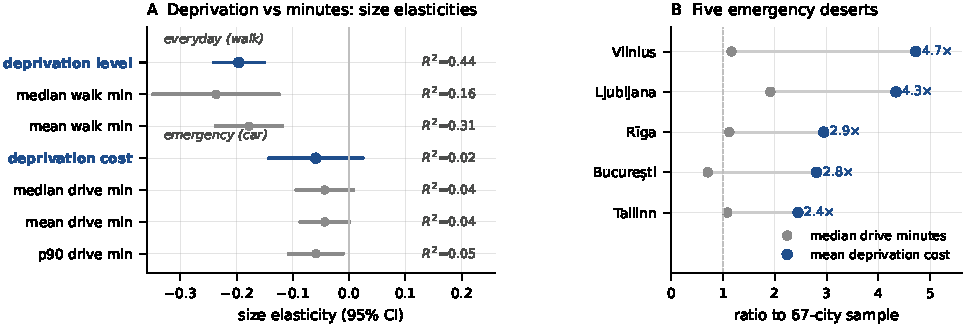
\includegraphics[width=\textwidth]{fig2_dep_vs_access.pdf}
\caption{Deprivation against access. (A) Size elasticities of
deprivation-based (blue) and minutes-based (grey) outcomes per regime
(95\,\% CIs, country-clustered). (B) The five emergency-desert capitals:
ratio to the 67-city sample under the access average (median drive
minutes) and under mean emergency deprivation cost. Sources: SI Appendix
Tables.}
\label{fig:depvsaccess}
\end{figure*}

\subsection*{Larger cities have lower everyday deprivation, but not lower
emergency deprivation}

If the returns to scale behind urban service provision were general
\citep{bettencourt2007growth,bettencourt2013origins}, both deprivations
should fall with city size. The everyday regime behaves as predicted
(Fig.~\ref{fig:scaling}A): the log-log elasticity of mean everyday
deprivation on population is $-0.196$ (country-clustered SE 0.023,
\pw{0.0002}), a fall of roughly 19\,\% per e-fold of population, and size
alone explains 44\,\% of the cross-city variance. The median walk to the nearest facility of each everyday category is
4--8 minutes, and larger cities carry denser networks. The estimate is stable
under country fixed effects, leave-one-out deletion, robust estimators,
exclusion of the desert capitals and a mapped-facility-density control
(SI Appendix).

The emergency regime breaks the pattern. The elasticity of mean emergency
deprivation cost is $-0.059$ (\pw{0.21}) and size explains 2\,\% of the
variance. Non-significance alone would be weak evidence, so the null is
bounded: two one-sided equivalence tests place the elasticity within
$\pm 0.13$ \citep{lakens2017equivalence}, and the minimum detectable
elasticity at 80\,\% power is 0.12, so the design could have found a
gradient of the everyday magnitude. The claim is ``no detectable scaling,
bounded within $\pm 0.13$'', never ``proven flat''. The median FUA has 6
emergency departments and 6 ambulance stations for its whole territory, a
median drive of 12 minutes to either, and the facility count of a
national emergency system does not multiply with population the way
pharmacies do. A paired regime test within cities puts the everyday slope
$0.137$ below the emergency slope (\pw{0.002}): agglomeration benefits
are regime-specific, and no single exponent describes what size does to
service deprivation. Size is not irrelevant to emergency deprivation,
however: a quadratic term is significant (wild $p = 0.001$), an inverted U
in which the middle strata carry the highest cost and the four largest
FUAs the lowest; with four cities in the top stratum we report the shape
and do not headline it (SI Appendix).

Within-city inequality moves the other way (Fig.~\ref{fig:scaling}B).
The Gini of everyday deprivation rises with population (elasticity
$+0.062$, \pw{0.0012}); the emergency Gini is size-flat at the baseline
($+0.004$, \pw{0.84}); the paired difference of $-0.058$ is significant
(\pw{0.029}). Size buys lower mean everyday deprivation at the price of a
wider spread around it, while emergency inequality is set elsewhere. The
everyday slope is positive under all 14 deprivation parameterisations and
significant in 13, the exception being the concave form swap ($+0.026$,
$p = 0.083$) \citep{simonsohn2020specification}. The emergency half is
conditional, and the conditionality is a finding: beyond the 15-minute
benchmark no clinical anchor exists, and there the three
literature-grounded escalation forms diverge (Fig.~\ref{fig:curves}C).
Under the bounded survival curve and under the polynomial baseline the
emergency Gini is size-flat, in agreement with the deprivation-free
travel-time Gini ($-0.015$, $p = 0.42$); under exponential escalation it
rises ($+0.098$, $p = 0.0003$), because exponential pricing turns the Gini
into an index of extreme-tail depth (SI Appendix). Two statements hold
under every parameterisation: everyday inequality rises with size, and
emergency inequality never falls with it.

\begin{figure*}[t]
\centering
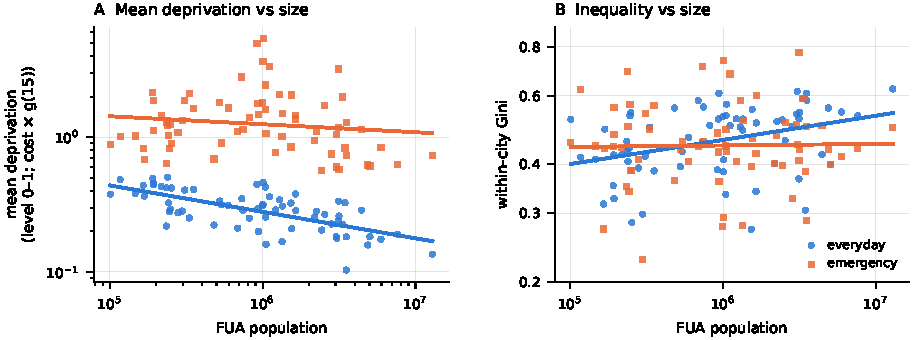
\includegraphics[width=\textwidth]{fig3_scaling.pdf}
\caption{What city size does to deprivation, per regime (log-log; 67
FUAs; cross-sectional). (A) Mean deprivation: everyday elasticity
$-0.196$ (wild $p = 0.0002$, $R^2 = 0.44$); emergency $-0.059$
($p = 0.21$, bounded within $\pm 0.13$); paired difference $+0.137$
($p = 0.002$). The two series are in different units and only the slopes
compare. (B) Within-city Gini: everyday elasticity $+0.062$
($p = 0.0012$); emergency $+0.004$ ($p = 0.84$); paired difference
$-0.058$ ($p = 0.029$).}
\label{fig:scaling}
\end{figure*}

\subsection*{Emergency deprivation follows national emergency-system
coverage, not city size}

City size explains 2\,\% of the variance in mean emergency deprivation
cost; 78\,\% lies at the country level (25\,\% between the four
macro-regions, 54\,\% between countries within regions), and the country
level also carries 70--76\,\% of the variance in both Ginis and their
gap (SI Appendix). We first identify the structure in the city vectors,
then its geography, then test it at the level at which it varies.

The 67 cities do not fall into types. k-means clustering on the full
standardised city vector separates 62 cities from 5 (silhouette 0.65,
bootstrap ARI 0.87, Gaussian-null $p = 0.001$), an outlier group with no
agreement with the region partition (ARI 0.001): the five desert
capitals, separated by their beyond-threshold emergency travel-time
tails. Ward clustering cuts the same axis more conservatively (65/2), and
re-clustering without the outliers finds one further cut along it, 48/14,
isolating partial-desert cities with real emergency tails (Oslo,
Stockholm, Warszawa, Sofia, Zagreb, Palermo and Luxembourg among them). The
nesting is evidence for a gradient, not types: a one-dimensional
\emph{coverage ordering} of the emergency periphery, covered (48),
partial desert (14), desert (5), robust to the feature set (ARI 1.00 and
0.97) with a soft boundary between covered and partial (SI Appendix). A
city's grade expresses how much of its population lives beyond the
emergency response benchmark. The grade, and no other variable we test,
sets the emergency level: in a country-clustered model with centred log
population, the grade dummies shift mean emergency deprivation cost
overwhelmingly (Wald $p \approx 10^{-15}$; median 1.02, 1.87 and 3.37
multiples of \gref{} across the three grades), while the slope-by-grade
interaction is boundary-sensitive and not headlined.

The ordering has a geography (Fig.~\ref{fig:geography}A). All five
deserts are capitals of Central-Eastern European (CEE) countries; the
partial-desert grade is a Nordic and CEE phenomenon (7 of 13 Nordic and 5
of 20 CEE cities, against 1 of 16 in the West and 1 of 18 in the South);
West and South are almost entirely covered. Grade and region are
different partitions and related: the emergency tail is a feature of the
sparse peripheries of Nordic FUAs and of the national emergency systems of
Central-Eastern Europe. In the inequality plane (Fig.~\ref{fig:geography}B)
the deserts are the five highest points on the emergency-Gini axis and
the partial deserts fill the band below them, so a city's emergency-side
inequality is, to a first approximation, its coverage grade. Across
cities the two Ginis are uncorrelated ($r = 0.12$, $p = 0.32$): how
unequally a city distributes everyday deprivation says nothing about how
unequally it distributes emergency deprivation, the cross-city face of
the two-regime claim.

Because macro-region is a property of countries, whole countries are
permuted across regions in every regional test. The emergency Gini
differs by region (Cohen $f = 0.74$, \pperm{0.0024}), as do the divergence
gap (\pperm{0.010}), the coupling $\rho$ of the two surfaces
(\pperm{0.0015}) and both compounding measures (\pperm{0.0008},
\pperm{0.0023}). Central-Eastern Europe compounds: the highest emergency
inequality (median Gini 0.54) with the strongest coupling (median
$\rho = 0.55$). Every CEE contrast survives re-testing without the five
deserts, and CEE's dispersion of the emergency Gini is about twice any
other region's (\pperm{0.028}). The everyday Gini's apparent regional
contrast does not survive country-level testing (\pperm{0.27}): the
Southern cities split by country, the Spanish cities and Athina at
0.50--0.61 against the Italian and Portuguese ones at 0.27--0.42, which
coincides with a known mapping artefact in general-practitioner tagging
(Limitations). The paper therefore makes no regional everyday-Gini claim
and no cross-country comparison of everyday levels.

\begin{figure*}[t]
\centering
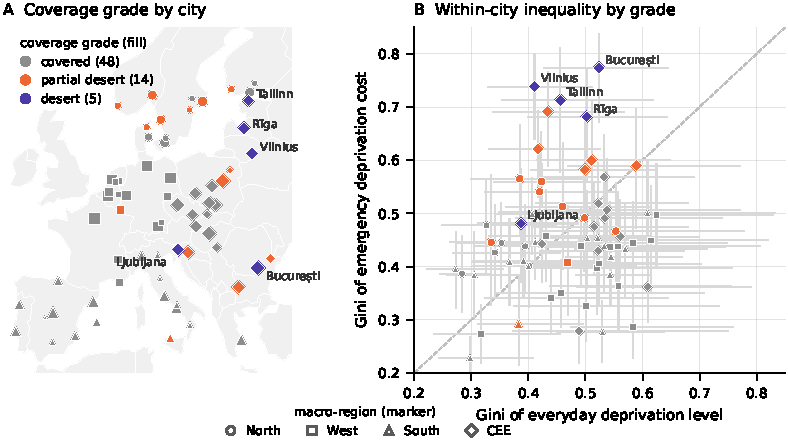
\includegraphics[width=\textwidth]{fig4_geography.pdf}
\caption{The geography of emergency coverage. (A) The 67 FUAs by coverage
grade (fill) and macro-region (marker), sized by population; the five
deserts are labelled. (B) Within-city Gini of the emergency deprivation
cost against the everyday level, same fill and markers; whiskers span the
min--max envelope of each Gini over the deprivation-curvature sweep.}
\label{fig:geography}
\end{figure*}

\subsection*{Compounding is the norm, and children carry it}

The co-location typology cuts both percentile surfaces at their
population-weighted medians, which fixes the marginals at one half; the
2$\times$2 class table then has a single free number, the high-high (HH)
compounding share, and statistical independence corresponds to
HH $= 25\,\%$. The observed share averages 33\,\% and exceeds independence
in 66 of 67 cities; the rank coupling $\rho$ spans $-0.02$ to $0.74$.
Compounding is not an exotic overlap of two rare conditions; across urban
Europe it is the default relationship between the two deprivations. The
``how high is high'' threshold moves the HH share 21 times more than the
whole deprivation calibration does, so the headline compounding measure
is the threshold-free intensity, the population-weighted mean depth to
which the typical resident sits inside both percentile distributions
(1/3 under independence); it shows the same regional structure. Spatially,
compounding concentrates in peripheries where the saturated everyday
level meets the escalating emergency cost, while dense cores hold most
population in the low-low class (all 67 maps in SI Appendix; per-cell
classes carry a 24\,\% routing-engine flip share and are read as patterns
only).

Who lives there? Following the social-vulnerability tradition
\citep{cutter2003vulnerability}, EU-harmonised census age strata are
pooled across all 67 cities, each compared against the cells where its
own census variable is published; national fine-grid strata are per-city
depth and never pooled. The result is one-sided (Fig.~\ref{fig:vuln}):
cells in the top quartile of child share carry more everyday deprivation
than their comparison cells in 88\,\% of cities (median ratio 1.27) and
more compounding in 88\,\% (median HH-share gap $+0.13$), strongest in
Central-Eastern Europe (1.44) and the North (1.30). The elderly show no
such pattern at the European level (median ratio 0.96, above parity in
37\,\% of cities), a null that is itself a result; national data resolve
sharper per-city patterns (in Hamburg, elderly 1.37, children 1.52,
low-rent 1.61) but stay per-city. The European claim is about children:
whatever sorting mechanism places families with children in the
compounded periphery operates across nearly the whole sample, in a group
whose daily radius is short and whose emergency risk is real.

\begin{figure}[t]
\centering
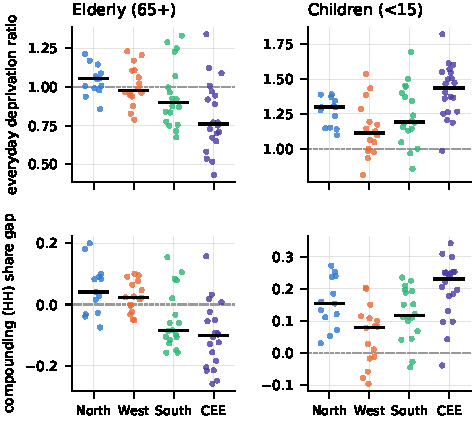
\includegraphics[width=\columnwidth]{fig5_vulnerability.pdf}
\caption{Who carries the deprivation. Census-harmonised strata by
macro-region, pooled across 67 cities against covered-cell references
(dashed: parity; bar: regional median). Top: everyday deprivation ratio;
bottom: compounding (HH) share gap. Children: higher everyday deprivation
in 88\,\% of cities (median 1.27) and higher compounding in 88\,\% (median
gap $+0.13$). Elderly: parity (0.96); no European elderly claim is made.}
\label{fig:vuln}
\end{figure}

% ==========================================================================
\section*{Discussion}
% ==========================================================================

\subsection*{Deprivation as the welfare measure of urban proximity}

The first contribution is to bring deprivation theory from humanitarian
logistics \citep{holguinveras2013objective,holguinveras2016econometric}
into the analysis of a functioning city. Where results are rank-based,
travel time and deprivation agree almost perfectly, which certifies the
accessibility literature's rank-level findings
\citep{nicoletti2023disadvantaged,wu2025global} at continental scale.
Where results concern levels, inequality magnitudes or tails, travel time
was never a welfare measure, and the divergence is not noise: the desert
capitals sit at 0.71--1.92 times the sample by access and 2.45--4.72
times it by deprivation, and the choice of measure decides whether an
emergency-side size story exists at all. The same limitation is conceded
from inside the resilience literature, where the latest building-level
frameworks measure access as network distance to the nearest facility
and note that distance captures one dimension of access only
\citep{pagancajigas2026acces}. The theory also explains why the two
regimes are different objects: a bounded level for substitutable needs
and an unbounded cost for time-critical needs are what it implies for the
two kinds of good, and the clinical response literature
\citep{larsen1993survival,nicholl2007distance} supplies the anchors that
a value of time estimated on reschedulable trips cannot. The framework
travels to any domain with anchors of comparable strength.

\subsection*{What urban growth delivers, regime by regime}

Scaling theory rests on exponents that hold across cities and quantities
\citep{bettencourt2007growth,bettencourt2013origins}; its refinements
condition them on the stage of a national urban system
\citep{musso2026cities}. Our results add a different condition: the
exponent depends on the regime of the service class, within one urban
system and one measurement. Everyday deprivation scales ($-0.196$,
44\,\% of variance); emergency deprivation does not (bounded within
$\pm 0.13$); the two slopes differ within cities. A single infrastructure
exponent is not a sufficient statistic for what size does to service
deprivation, and in a mature urban system, where large cities no longer
grow faster than small ones \citep{musso2026cities}, what size still
delivers is lower everyday deprivation. The inequality result cuts
deeper: everyday inequality rises with size under every parameterisation,
so the agglomeration that lowers mean everyday deprivation widens its
spread, which argues that the scaling of within-city, welfare-weighted
distributions is where the next generation of scaling laws has to live.
The 15-minute-city paradigm \citep{moreno2021fifteenminute,allam2022fifteenminute}
emerges recast: its threshold anchors the everyday regime well, and
precisely because that regime saturates, a proximity paradigm is an
everyday-services paradigm, silent about the escalating-cost regime and
about the populations where both fail.

\subsection*{Built for the everyday, tested by the emergency}

Resilience research defines resilience through equitable access to
essential services \citep{logan2020reframing,meerow2016defining}, finds
that access equality and network resilience reinforce each other
\citep{fan2022equality}, and shows everyday vulnerability failing to
predict crisis capability \citep{sirenko2026heatwaves}. Our two-regime
measurement gives that distinction quantitative form across an urban
system: the everyday surface is set by the city and its density, the
emergency surface by the coverage of a national emergency system, so a
city's resilience cannot be read from either alone, and a city built for
the everyday regime is not thereby resilient. Compounding is the case the
coupled-systems argument predicts: the same neighbourhoods in the
periphery of both systems, above independence in 66 of 67 cities,
strongest where emergency inequality is highest, and consistently the
neighbourhoods with many children. The measurement is of the emergency
regime under normal conditions, the floor from which any disruption
starts. Frameworks that predict building-level loss of access after a
hazard take a pre-hazard baseline of network distance to the nearest
operational facility as their starting point \citep{pagancajigas2026acces};
the emergency-deprivation geography measured here is that baseline for
urban Europe, in welfare terms, and it matters more each year as heat
exposure and heat mortality rise \citep{naumann2020heat,garcialeon2024mortality}
and the Preparedness Union Strategy asks member states to plan hospitals,
schools and transport for the emergency regime \citep{ec2025preparedness}.
The practical reading follows the two jurisdictions. Everyday inequality
is a big-city problem: it rises with size, and intra-urban service
planning is the lever. Emergency deprivation is a national coverage
problem: it follows coverage grade rather than size, and its extreme
cases are five capitals whose peripheries no municipal instrument can
serve alone; the coverage ordering is a screening variable access
averages do not provide. The consistent carriers of compounded
deprivation are families with children, which makes school- and
family-anchored service planning a compounding remedy rather than a
sectoral one.

\subsection*{Limitations}

Every size gradient is cross-sectional. The analysis covers walking for
everyday services and driving for emergency care; public transit is out
of scope by design. Free-flow civilian drive times anchor the emergency
cost scale and are not response-time predictions; congestion lengthens
drive times most in the largest cities, so free-flow routing understates
emergency deprivation there and pushes the emergency elasticity toward a
size benefit, which makes the absence of a gradient a conservative
finding. Disruption itself is not modelled, so the emergency surface is
the pre-disruption baseline that hazard-specific frameworks perturb
\citep{pagancajigas2026acces}. Census strata are 1\,km attributes
broadcast to the 100\,m grid. Per-cell typology classes carry a roughly
24\,\% routing-engine flip share and are read only as patterns. The
deprivation layer itself is the first thing a reader should attack, and
SI Appendix reports the attack in full: levels move with the calibration
and are meant to, while ranks and classes do not. Mapped
general-practitioner density varies about 12-fold across countries in a
way that reflects OpenStreetMap tagging conventions rather than health
systems, which overstates everyday deprivation levels in the Nordic and
Southern countries; cross-country everyday level comparisons are therefore
not supported, while the size gradients are unaffected (mapped density is
uncorrelated with size, and a density control leaves the elasticities in
place). Eight cities have only one of the two emergency services mapped;
none is in the desert group and no headline turns on it (SI Appendix).

% ==========================================================================
\section*{Materials and Methods}
% ==========================================================================

\subsection*{Design and sample}
The study is a cross-sectional comparison of 67 FUAs in 24 countries under
one harmonised city definition, the Eurostat--OECD functional urban area
\citep{dijkstra2019fua}, with trajectories read from the cross-sectional
size gradient as in \citep{musso2026cities}; there is no longitudinal
component. The sample is a stratified draw over four macro-regions and
four population strata (100{,}000--250{,}000; 250{,}000--1 million; 1--5
million; above 5 million; 15/18/30/4 cities), seeded once and fixed
before any surface was computed. Countries nest inside regions, and every
cross-city test is built around that nesting.

\subsection*{Data and travel times}
The analysis unit is the populated 100\,m cell of the GHS-POP R2023A grid
\citep{schiavina2023ghspop}, clipped to each FUA; every aggregate is
population-weighted. Facilities come from OpenStreetMap under one tag
taxonomy: five everyday categories reached on foot (general
practitioners, pharmacies, supermarkets, schools, green spaces) and two
emergency services reached by car (emergency departments, ambulance
stations); median counts per FUA are 93, 228, 325, 409, 636, 6 and 6.
Travel times are routed with R5 \citep{fink2022r5py} over the
OpenStreetMap network, walking at 4.8\,km/h with a 30-minute cut-off and
driving at free-flow speed with a 60-minute cut-off, from facilities to
cells and transposed (median car asymmetry one minute; the transposed
direction is the correct one for ambulance response). Cells with no
network path are masked under one shared mask; cells that are routable
but beyond a service's cut-off receive a large finite time so that the
everyday level saturates and the cell stays on the map. Census strata come
from the Eurostat Census 2021 1\,km grid (harmonised age groups) and,
where published, national fine grids; withheld counts are missing, never
zero. A friction-surface engine \citep{weiss2020healthcare} is a declared
sensitivity variant after a two-city cross-check showed city-specific
level bias (SI Appendix).

\subsection*{Deprivation functions}
In both regimes the functional form is transferred from the estimated
literature and the curvature calibrated to domain anchors, because the
published coefficients were estimated on hours of deprivation and do not
transfer to intra-urban minutes. For each everyday service, travel times
to reachable facilities are adjusted for congestion by a two-step floating
catchment area factor \citep{luo2003measures,luo2009enhanced} and reduced
by a soft minimum,
$t^{\mathrm{eff}}_{is} = -\kappa^{-1}\ln\sum_j \exp(-\kappa\, t_{ij} c_j)$,
so that several similar options count as slightly closer than the nearest
alone. The everyday deprivation level is the logistic
\begin{equation}
D_{is} = \big[1 + \exp(-k\,(t^{\mathrm{eff}}_{is} - t_0))\big]^{-1},
\quad t_0 = 15\ \mathrm{min},\ k = 0.2\ \mathrm{min}^{-1},
\end{equation}
the saturating S-curve of needs-based severity \citep{wang2017deprivation}
with its inflection at the 15-minute-city threshold
\citep{moreno2021fifteenminute}, averaged over the service categories
reachable from the cell. The emergency deprivation cost uses the nearest
facility and a convex Box-Cox function
\citep{cantillo2018discrete,delgadolindeman2019ambulance},
\begin{equation}
C_i = \frac{g(\min_j t_{ij})}{g(15)}, \qquad
g(t) = \frac{(t+1)^{\lambda} - 1}{\lambda}, \quad \lambda = 1.8,
\end{equation}
anchored on the EMS response benchmarks: negligible below the 3--4 minute
ideal \citep{pons2005response,vo2020vulnerable}, about a third of the
benchmark cost at the contested 8-minute standard
\citep{pons2005response,blanchard2012response,khan2026melbourne}, and
equal to it at the 15-minute upper target \citep{peleg2004ems}, with
convexity supported by distance-mortality evidence
\citep{nicholl2007distance}. Solving $\lambda$ from the anchors gives
1.89--1.95, inside the sensitivity sweep. Division by $g(15)$ reports
costs in multiples of the benchmark deprivation and leaves every
rank-based statistic and both Ginis unchanged.

\subsection*{Indicators and cross-regime comparison}
Only unit-invariant statistics cross regimes: elasticities, the
population-weighted within-city Gini (mean-normalised, so comparing the
inequality of a level with that of a cost is the move of comparing an
income with a wealth Gini) and rank statistics on the population-weighted
mid-rank percentile of each surface. The co-location typology cuts both
percentile surfaces at their medians; at that split
$\mathrm{HL} = \mathrm{LH} = 0.5 - \mathrm{HH}$ and
$\mathrm{LL} = \mathrm{HH}$, so the HH share is the one free number and
independence gives 0.25. Alongside it we report the Spearman coupling
$\rho$ of the two percentile surfaces and the threshold-free compounding
intensity, the population-weighted mean of $\min(p^{\mathrm{ev}}_i,
p^{\mathrm{em}}_i)$, which equals 1/3 under independence and 1/2 under
perfect coupling. Vulnerability strata (top quartile of child share, of
share aged 65 and over) are compared against the cells where their own
variable is published; strata covering less than half a city's population
are dropped from the pooled summary.

\subsection*{Inference}
Each outcome is regressed as $\ln y_c = \alpha + \beta \ln P_c +
\varepsilon_c$ \citep{bettencourt2007growth}, with standard errors
clustered on country and a wild cluster bootstrap p-value with the null
imposed (Rademacher weights, 4{,}999 draws)
\citep{cameron2008bootstrap,mackinnon2023cluster}. The emergency null is
bounded by two one-sided equivalence tests \citep{lakens2017equivalence};
the regime difference is tested within cities by a regime $\times$
log-population interaction; every headline elasticity carries
leave-one-out, Cook's-distance, Huber and median-regression diagnostics, a
mapped-facility-density control and quadratic and stratum-dummy
non-linearity checks. Regional contrasts compare country means and
permute whole countries across regions (10{,}000 permutations); the
city-level ANOVA is an anti-conservative reference. A nested
sum-of-squares decomposition, a Fligner--Killeen dispersion test under the
same permutation, and re-tests without the desert capitals characterise
where the variance lies. Clustering runs k-means and Ward on the
robust-scaled city vector with $k$ selected by silhouette, each partition
carrying silhouette, bootstrap adjusted Rand index, a Gaussian silhouette
null and the ARI against the region partition; when the winning split
isolates an outlier group a peeled second pass re-clusters the rest, and
the coverage grade is read off the two passes, never from a hand-set
threshold. A structured sensitivity sweep varies curvature
($k \in \{0.1,0.2,0.3\}$, $t_0 \in \{10,15,20\}$, $\lambda \in
\{1.4,1.8,2.2\}$), swaps the functional forms while pinning the same
anchors, sweeps the accessibility model and the typology threshold, and
reports rank agreement, envelopes, flip-cell shares and the
specification curve of the inequality slopes over all 14
parameterisations \citep{simonsohn2020specification}. Full procedures,
including the reachability split, the robustness layers and the
routing-engine cross-check, are in SI Appendix.

\subsection*{Data and code availability}
All tables and figures trace to the persisted 67-city state; every quoted
number is checked against its source table by an automated audit of 190
checks run in continuous integration. Code, configuration, result tables,
per-city maps and sensitivity sweeps are available in the study
repository and its results branch. Population grid: GHS-POP R2023A.
Facilities and networks: OpenStreetMap. Census strata: Eurostat Census
2021 grid; German Zensus 2022 grid. Boundaries: Eurostat--OECD functional
urban areas.

\bibliographystyle{unsrtnat}
\bibliography{../references}

\end{document}
